\chapter{文献综述}

\section{背景介绍}

\indent 行人再识别(Person Re-identification,简称ReID), 也称行人重识别\cite{zheng2016person},如图~\ref{figure:background},是利用计算机视觉技术,在图像或者视频集合(gallery)中找到与询问图片(query)相似行人的任务。理论上来说,视频监控中的行人再识别系统应该被分解为三个子模块:行人检测、行人跟踪、行人检索。前两个模块是计算机视觉中已经存在的任务,因此大多研究者所指的行人再识别问题着力解决行人检索问题\cite{zheng2017person}。本文也不例外,着力解决光照、姿态、视角急剧变化下的行人再识别/检索问题。

\begin{figure}
	\centering
	\captionsetup{width=.88\linewidth}
	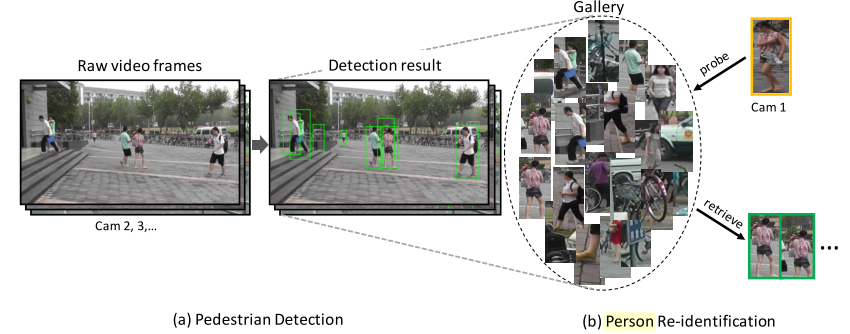
\includegraphics[width=\linewidth,keepaspectratio]{data/kaitibaogao/background.png}
	\caption{\kaiti 典型行人再识别系统的流程,整个行人再识别系统包括:视频行人检测、行人跟踪、行人检索。目前的工作主要集中在行人检索问题上。因此大多研究者所指的行人再识别问提指的是其中的子模块——行人检索问题。}
	\label{figure:background}
\end{figure}

行人再识别中存在许多挑战。由于行人的非刚性运动、检测器的误差、摄像头的视角变化,同一行人的不同图片往往存在严重的空间失配(Spatial Misalignment);行人没有可靠的生物特征,只能从属性、语义层面的特征加以区分;未标定的摄像机参数、巨大的时空跨度,这些都进一步增加了再识别的难度;同时现有的数据集规模相对较小,不存在ImageNet或者MegaFace这样的大规模、可以泛化迁移(Transfer)到任意子领域(domain)的数据集。这导致数据集间存在较大偏差(domain bias/domain shift),从一个数据集到另一个数据集,模型的性能通常都会下降。

\section{国内外研究现状}

由于行人再识别的应用和研究的价值,他在计算机视觉领域受到了越来越多的关注和巨大的发展。近几年,再识别领域投稿数量增加,性能也呈指数增长,2015年好的模型cmc-1(Cumulative Matching Characteristic)只有$65\%$。17年在$80\%-85\%$。但是在17年短短11月,Arxiv上公布的文章已经达到了$90\%-96\%$。18年行人再识别领域的cmc-1已经能够在大型数据集上超越人类的表现。
目前的研究者大多从几个固定的方面深入研究。从损失函数分类上看,行人再识别主要使用分类损失、度量损失,分别对应表征学习和度量学习。这是再识别的基本方法,在此基础上,国内外的研究者往往从特征学习、网络结构的设计(如引入结构先验——行人由几个部分构成、具有相对空间位置关系)或者提出新的问题(视频再识别、生成数据、大规模检索、弱监督学习)等方面着手。本综述也将从这些方面展开。

\subsection{表征学习与度量学习}

\textbf{表征学习(Representation learning):}通过转化为分类(Classification/ Identification)问题或者验证(Verification)问题,进行监督性学习训练,取全连接层的特征作为很好的表征。之所以说是很好的表征,是因为输入图片原本线性不可分,但是最后一层线性分类层的特征变得线性可分,从而使得后续任务变得简单。w无论是分类还是验证问题,在转化之后,会使用softmax作为激活函数。在有的论文中,作者认为光靠行人的ID信息不足以学习出一个泛化能力足够强的模型,于是额外标注了行人图片的属性特征,例如性别、头发、衣着等属性。通过引入行人属性标签,模型不但要准确地预测出行人ID,还要预测出各项正确的行人属性。

\textbf{度量学习(Metric learning):}度量学习广泛应用于图像检索。不同于表征学习,度量学习通过设计距离度量函数,直接学习特征。优化目标直接就是同一行人不同图片特征之间的相似度更小,不同行人的更大。损失函数使得相同行人图片(正样本对)的距离尽可能小,不同行人图片(负样本对)的距离尽可能大。常用的度量学习损失方法有对比损失(Contrastive loss) \cite{varior2016gated}、三元组损失(Triplet loss)、四元组损失(Quadruplet loss)、难样本采样三元组损失(Triplet hard loss with batch hard mining, TriHard loss)\cite{hermans2017defense}、边界挖掘损失(Margin sample mining loss, MSML)

两者最终学到的特征,都是语义上紧凑的表示,能够根据ID聚成不同的类别,有利于后续任务的进行。但是区别在于表征学习是通过定义其他有关联的分类任务间接学到表征的。

\begin{figure}
	\centering
	\captionsetup{width=.88\textwidth}
	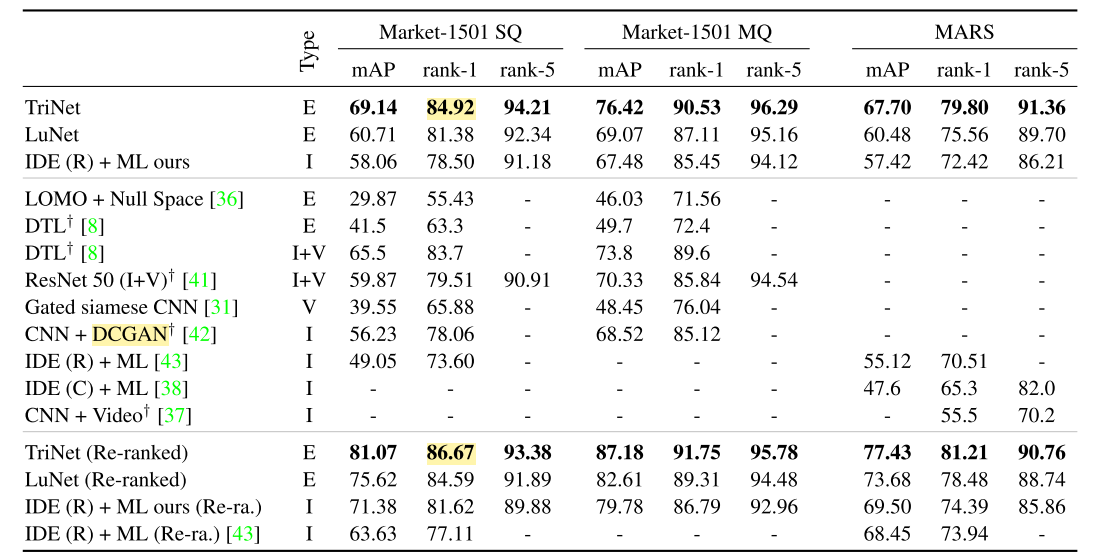
\includegraphics[width=\linewidth,keepaspectratio]{data/kaitibaogao/loss-perf.png}
	\caption{\kaiti 表示学习、度量学习的方法比较,其中,TriHard方法获得了最好的效果。在不使用Rerank后处理的情况下,得到了84.92的rank-1指标,在rerank和使用multi-shot查询的情况下,获得了91.75的rank-1指标。}
	\label{figure:loss}
\end{figure}

表征学习实现简单,当每个ID都有充足的训练图片时效果很有竞争力。如图~\ref{figure:loss},实践证明,在行人再识别、人脸验证这一类问题,度量学习只要训练得当,就能够获得更快的收敛速度与泛化能力。因此,本节将重点叙述表征学习的方法。

对比损失用于训练孪生网络(Siamese network),网络含有两条分支,三元损失用于训练三条分支的网络。但是由于各条分支之间参数共享,所以可以使用一条分支高效实现。首先介绍对比损失,假设输入图像a和b,提取到的特征之间的距离定义为
\begin{equation} {d_{a,b}} = \left\|{f_{{I_a}}} - {f_{{I_b}}}\right\|{^2}\end{equation}

当两张图属于同一行人时,标签y=1,不同行人时,标签y=0,则对比损失为
\begin{equation} {L_c} = yd_{a,b}^2 + (1 - y)(\alpha  - {d_{a,b}})_+^2\end{equation}

三元损失的三个输入分别为锚定图片(Anchor) a ,正样本图片(Positive) p和负样本图片(Negative) n。图片 a 和图片 p 为一对正样本对,图片 a 和图片 n 为一对负样本对。三元组损失表示为:
\begin{equation} {L_t} = {({d_{a,p}} - {d_{a,n}} + \alpha )_ + }\end{equation}

传统的三元组随机从训练数据中抽样三张图片,由于随机抽取的往往是无用信息,导致训练时间长、收敛慢,而且容易训练崩塌。因而长期以来,研究者普遍认为使用度量损失往往比表示学习中的分类验证损失效果差。\cite{liu2017quality}提出了一种基于训练批量(Batch)的在线难样本采样方法——TriHard Loss,比所有17年所有的最新方法性能和收敛速度都好了一大截。
对于每一个训练batch,随机挑选 P 个ID的行人,每个行人随机挑选 K 张不同的图片,即一个batch含有 $P\times K$ 张图片。之后对于batch中的每一张图片 a ,我们可以挑选一个最难的正样本和一个最难的负样本和 a 组成一个三元组。

我们定义和a 具有相同ID的图片集为 A,剩下不同ID的图片图片集为 B,则TriHard损失表示为:
\begin{equation}
	L_t=\frac{1}{PK}\sum_{a \in batch} \left( \max_{p \in A} d_{a,p} -  \min_{n \in B} d_{a,n} +\alpha \right)_+
\end{equation}

\subsection{融合局部特征}

在行人再识别中,一个很热门的研究方向就是提取更好的局部特征\cite{reciprocal,liu2017hydraplus,zhao2017spindle,glad},18年性能很高的几篇论文基本上都使用了局部特征\cite{liu2017hydraplus,zhao2017spindle}。其中对齐再识别\cite{zhang2017align}使用最短路径自动匹配局部特征,算法复杂度较高,通过辅助全局特征的训练获得了超过人类的表现,详细可以参考文献翻译。

上下文特征\cite{latent}使用STN结合先验定位可变性的行人部分,从原始图片中预测定位参数,从而便于后续的网络将注意力集中于具有潜在语义的身体部分。考虑到视频监控环境下行人的姿态先验——行人通常直立于地面,作者使用了4个自由度的仿射变换矩阵,建模了尺度、平移方面的可变性变换。
\begin{equation}
	\left(\begin{array}{c}
			x^{in}_i \\
			y^{in}_i
		\end{array}\right) =\left[ \begin{array}{ccc}
			s_x & 0   & t_x \\
			0   & s_y & t_y
		\end{array}\right] \left(\begin{array}{c}
			x^{out}_{i} \\
			y^{out}_i   \\
			1
		\end{array}\right)
\end{equation}

由于具有了可变性的特性,学到的身体部分能够减轻视角和背景带来的类内差异。但是由于随机生成的反射矩阵参数会产生巨大形变,作者不得不增加正则项将其限制于先验的附近。最终将全局特征与身体各部分的特征融合,结合分类损失训练。

\subsection{GAN生成样本}

如图~\ref{figure:dataset}所示,ReID有一个非常大的问题就是数据获取困难,截止CVPR18 deadline截稿之前,最大的ReID数据集只有1k ID,36k 图片。视频数据集的图片数量当然达到上万,但是冗余较高,有效的图片仍然少于几千张。因此,使用gan生成图片提升泛化能力显得非常重要。

\begin{figure}
	\centering
	\captionsetup{width=.88\linewidth}
	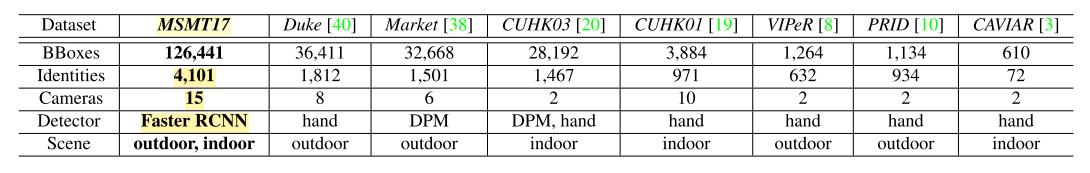
\includegraphics[width=\linewidth,keepaspectratio]{data/kaitibaogao/dataset.png}
	\caption{\kaiti ReID常用数据集统计信息,可以看见,ReID领域公开数据集规模通常较小}
	\label{figure:dataset}
\end{figure}

试管实验一文\cite{zheng2017unlabeled}是第一篇用GAN做ReID的文章,由于生成的图像质量较差,没有明确的id信息,论文使用的是标签平滑的方法,将label vector每一个元素的值取为各个类别的均匀分布。生成的图像作为训练数据加入到训练之中,相当于在训练过程中引入了适当的噪声,避免了过拟合提升了泛化能力。

在此基础上,姿态归一化一文\cite{qian2017pose}提出了改进,一方面能够相同ID的行人,另一方面克服了行人姿态不同带来的类内差异。

\begin{figure}
	\centering
	\captionsetup{width=.88\linewidth}
	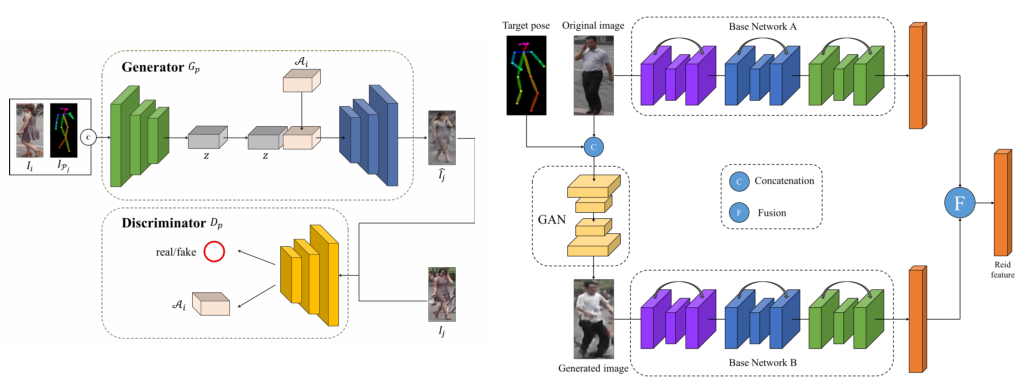
\includegraphics[width=\linewidth,keepaspectratio]{data/kaitibaogao/pose-norm.png}
	\caption{\kaiti 姿态归一化一文\cite{qian2017pose}所使用的网络结构。左图:最终网络结构——原始图片提取特征与姿态归一化后图片提取的特征融合,用于再识别。右图:生成姿态归一化图片的GAN网络结构,融合姿态、ID、属性等信息,生成较高质量的图片。}
	\label{figure:pose-norm}
\end{figure}

论文首先使用在coco上预训练的pose estimation网络提取骨骼关键点,由于数据集之间存在偏差,往往存在很高的误检漏检。将pose信息和原图共同作为条件信息,输入pixel2pixel网络,并使用属性和ID作为额外的监督信息,将原本无监督的GAN生成问题转化为半监督学习,生成了质量较好的行人图片。作者选取了8个视角,通过GAN将single query转化为了multi query,通过max-pool形式,将不同视角的行人图片提取的特征与baseline网络提取的特征融合。

最终在Market1501上再次获得了超过人类表现的性能,获得了95.52\%的rank-1指标,在CUHK03上也获得了不错的性能。在CUHK03上性能没有超过人类的原因在于,属性标签只在Marke1501有标注,泛化到CUHK03上反而会由于数据集的偏差降低性能。同时该方法在半监督学习的设置下也获得了很好的效果,不使用目标数据集调优,在VIPeR小数据集上直接得到了68.67\%的rank-1指标。

\begin{figure}
	\centering
	\captionsetup{width=.88\linewidth}
	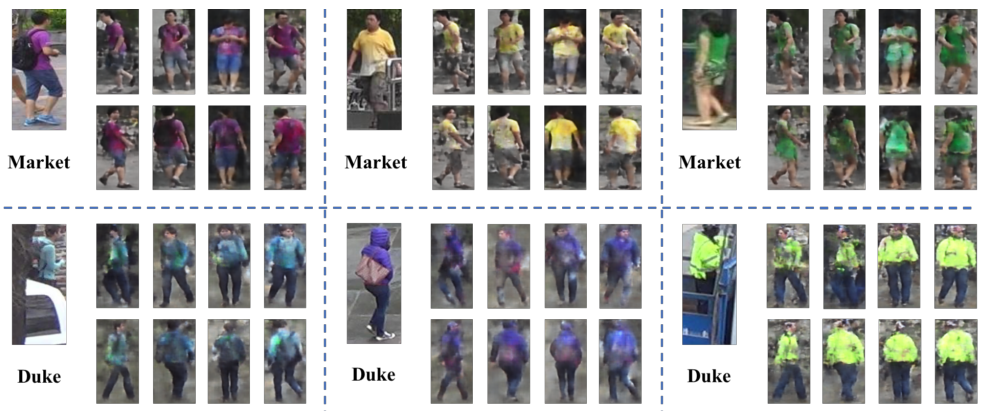
\includegraphics[width=\linewidth,keepaspectratio]{data/kaitibaogao/vis.png}
	\caption{\kaiti 在Market1501和DukeMTMC-reID数据集上生成图片的效果。}
	\label{figure:vis}
\end{figure}

\section{其他方向}

目前视觉领域逐渐开始从图片转向了视频,对于再识别而言,两者最大的区别在于询问视频序列具有多张图片。对此,常用的有两种方案:多张query图片多次查询,聚合排序结果;聚合查询图片的特征,然后只进行一次查询。两种方法相比,后者在大规模检索问题中更具实用性和扩展性。因此再识别领域往往借鉴视频动作识别中的想法将多张图片的特征聚合。比如捕捉特征随时间的演化模式、通过在CNN中嵌入三维卷积直接得到视频级别的特征描述。

累计运动背景网络(Accumulative motion context network, AMOC)\cite{liu2017video}使用视频动作识别中效果最好的双流网络提取空间特征和光流(运动)特征,融合后输入到一个RNN来提取时序特征。其中,由于光流运动信息的提取非常耗时,作者首先训练了一个类似U-Net结构的运动信息网络,输入原始图像序列,前馈网络预测不同尺度的光流图像拼接为最终的预测光流。通过AMOC网络,每个图像序列都能被提取出一个融合了内容信息、运动信息的特征。网络采用了分类损失和对比损失来训练模型。融合了运动信息的序列图像特征能够提高行人重识别的准确度。

\begin{figure}
	\centering
	\captionsetup{width=.88\linewidth}
	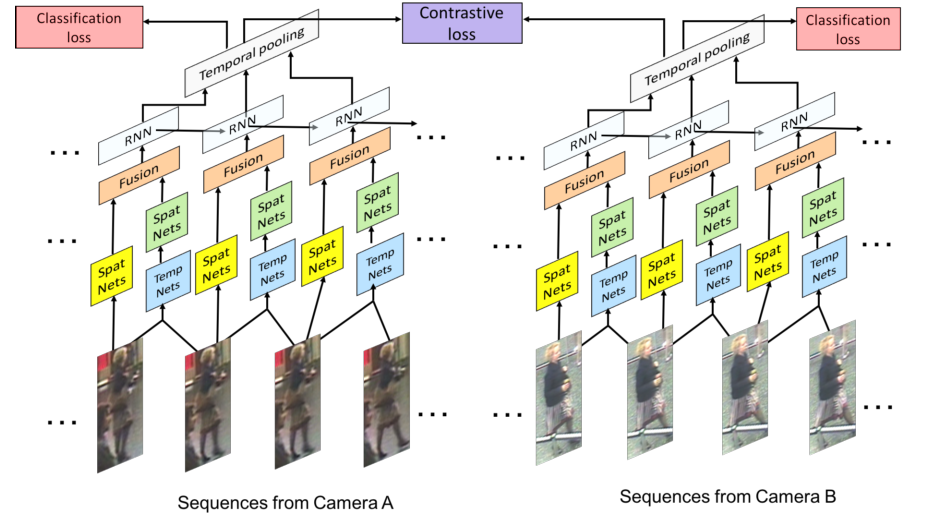
\includegraphics[width=\linewidth,keepaspectratio]{data/kaitibaogao/motion.png}
	\caption{\kaiti 累计运动背景网络结构}
	\label{figure:motion}
\end{figure}

另一方面,行人再识别领域的gallery集合中图片数量不断扩大,从传统数据集的100k增长到了500k,开始逐渐迈向大规模检索的现实场景。随着gallery集合的增大,会带来两方面的挑战:性能的下降和速度的下降。

性能方面,由于迷惑项的增加,mAP降幅最大可达7\%。同时为了达到实时的速度,在性能与速度的权衡后,我们往往采用近似最近邻搜索,牺牲一定的精度,导致性能进一步下降。

速度方面,我们非常需要紧凑的特征表达,将一张图片映射到2048维的语义空间和128维的语义空间,在距离矩阵的计算速度上会有巨大差别。从500k到10M的gallery集合,耗时会增加60.7s!于是我们有必要从图像检索领域借鉴想法。但是与图像检索有所区别的是,在训练阶段再识别问题被标注有ID信息,可以作为分类问题;而在测试阶段,再识别问题完全变成了检索问题。除了算法上存在难题,数据集上也还没有达到图像检索的规模。于是近期,悉尼大学的学者将会提出一个具有更多迷惑项、强调检索实时性的行人再识别数据集。


\bibliographystyle{data/gbt7714-2005}
{
	\renewcommand{\chapter}[2]{\section{#2}
	% \addcontentsline{toc}{section}{#2}
	}
	\bibliography{data/kaitibaogao}
}

% 按文章长度需要启用
\ifthenelse{\equal{\zjuside}{T}}{\newpage\mbox{}\thispagestyle{empty}}{}

\chapter{开题报告}

\section{研究开发的背景、意义与目的}

\subsection{背景介绍}

大多数研究者所指的行人再识别目标是跨摄像头识别同一行人[4]。由于姿态、遮挡和背景干扰的存在,再识别任务急需一种强大的特征表示,具有较小的类内间距和较大的类间间距。对此,我们可以从全局特征、局部特征的融合,或者采用全新的训练方式,提升特征的鲁棒性和表达能力。

\subsection{本研究的意义和目的}

从多个角度研究行人再识别,通过广泛阅读行人再识别方面的文献和动手实验,了解行人再识别中真正有用的关键技术。同时也阅读相关领域的论文,行人再识别领域一个很明显的趋势就是不停地从其他领域借鉴新问题和新方法,从人脸验证到图像检索再到信息检索(数据挖掘)。目前人脸验证中的开放环境验证(Open-set Verification)、各种loss函数、使用GAN生成多视角的样本,图像检索中的迷惑图片(Distractor)、大规模信息检索中速度与精度的权衡、可缩减的特征表示[2]、rerank后处理[3]等思路都已经引入行人再识别。信息检索、web搜索中还有一些概念可能还没有引入,比如专家(Expert/Local Model)、社区(Community)。
最后还可以进行的方向包括:结合认知科学中对人类视觉皮层结构的研究成果,提出可变性(Deformable)、动态(Dynamic、Running Time)的模块,提取鲁棒的特征,利用结合IRGAN利用对抗网络挖掘最具竞争力的样本,利用强化学习选择最富有信息的样本,使用记忆网络摒弃所有point2point的方法将set2set的问题[10]真正地解决。
我们也将从行人再识别的各个方面着手,先达到State of the Art的效果,再尝试提出自己的想法。

\section{主要研究开发内容}

\subsection{主要研究内容}

主要研究行人再识别中的起作用的关键技术。包括再识别中的基础技术:siamese network、match network、histogram特征的提取,再识别中起作用的技术:Triplet loss、online hard negative mining、rerank后处理,以及最后在IRGAN、NTM方面继续尝试。

\subsection{技术路线}

从基本方法开始,首先熟悉再识别数据集和任务,然后尝试复现达到最新论文的效果,最后基于之前积累的经验,选择几个最有可能成功的方向,提出想法、进行试验从而能有自己的创新。

\subsection{可行性分析}

分为三个阶段,从熟悉再识别任务,到复现最新方法,再到提出自己的方法,前面两个阶段比较基础,最后一个阶段具有挑战性。
针对发表论文的目标而言,这样的技术路线是否可行?从研究的问题上来说,行人再识别作为新兴的研究方向投稿论文增加,本身课题具有可行性;从使用的方法上来说,我们可能会采用IRGAN、RL、GAN、NTM等方法,或者提出一些基础通用的模型,具有可行性。

针对学习最新方法的目标而言,这样的技术路线是否可行?一方面,我们直接从开源代码、文档、最新论文着手,可以在最短时间内掌握一个最前沿的方向。另一方面,虽然我们没有时间系统阅读Deep Learning、Reinforcement Learning: An Introduction、Element Of Statistics Learning或者学习一些公开课,系统地了解深度学习领域的知识,但是我们会取长补短,仔细选择和仔细阅读相关部分论文,方便撰写论文。具有可行性。

\section{进度安排及预期目标}

\subsection{进度安排}

\subsubsection{熟悉典型的行人再识别数据集}

行人再识别中大型的数据集包括CUHK03、Market1501,每个数据集都有自己强调的创新之处,比如CUHK03强调图片数量和行人数目是15年最多的数据集,Market1501在此基础上强调使用DPM检测器,图片质量具有自然场景下应有的噪声与挑战。比较不同的数据集主要可以从行人ID数据、图片数据、训练测试数量、gallery集合大小、数据质量方面衡量。这一阶段,重点掌握各个数据集的共性,准备好各个数据集调用的同一接口,从而方便之后的研究对比实验。

\begin{table}[!htbp]
	\centering
	\captionsetup{width=.88\linewidth}
	\caption{\kaiti 常用数据集的统计特性}
	\label{table:dataset}
	\begin{tabular}{|l||l|l||l||l|l|}
		\hline
		cuhk03.combine & \#ids & \#images & market1501 & \#ids & \#images \\ \hline \hline
		train          & 1267  & 12183    & train      & 651   & 11281    \\ \hline
		val            & 100   & 948      & val        & 100   & 1655     \\ \hline
		trainval       & 1367  & 13131    & trainval   & 751   & 12936    \\ \hline
		query          & 100   & 965      & query      & 750   & 16483    \\ \hline
		gallery        & 100   & 965      & gallery    & 751   & 19281    \\ \hline
	\end{tabular}
\end{table}

当然目前行人再识别领域数据集频出,各种新的任务也不断出现。传统的CUHK01、VIPeR通常只在弱监督、迁移学习中会被研究和使用。视频ReID任务常常使用PRID 2011,iLIDS-VID和MARS。为了衡量每帧图片质量,Sensetime新推出了Labeled Pedestrian in the Wild (LPW)数据集,其中包含7,694个tracklets,超过590,000个图片。为了衡量现实场景下行人搜索任务的性能,悉尼大学的Zheng Liang提出了PRW数据集。为了研究迁移学习,比现有数据集规模再大3.5倍的MSMT17即将开源,该数据集在时空跨度、行人多样性、背景干扰方面的挑战更大。如果有余力,也可以整理一下这方面的数据接口,有助于将来进行Ablation Study。

\subsubsection{广泛阅读文献,熟悉典型的行人再识别方法}

使用CNN做行人再识别的典型方法包括:改进的行人再识别(ImprovedReID)、基于深度语义特征的行人再识别(DCSL)、基于行人局部特征的行人再识别(Part-reid)。
从这些方面的论文着手,了解以前和现在的研究者对行人再识别常用方法存在怎么样的理解、分类甚至偏见。比如悉尼大学的Zheng Liang观察到当每个ID的训练样本达到10张以上时,基于identification方法(IDE,identity discriminative embedding)的模型能很轻松地实现高准确率,而基于Siamese模型的Verification方法,每次只能看见两个样本判断相似与否,难以完全利用所有ID的标注信息。因而该组的学者后续提出的方法的baseline都是IDE模型。这种方法简单有效,但是该组学者没有探索通过挖掘富有信息的样本尽可能利用所有ID标注信息,提升模型泛化能力的方法。因而,我们需要广泛阅读世界各地研究者对再识别的见解,获得全方位的了解。

\subsubsection{通过实验熟悉行人再识别方法,复现最新工作}

TriHard、Part-reid等方法都有开源代码,我们会基于这些工作进行实验,复现最新工作的效果。第一步,通过实验,理解这些方法为什么能起作用,存在什么缺点。
现有模型往往在较小随机选择的训练集子集上达到近乎完美的效果(cmc-1为99\%),但是在测试集上泛化能力不佳(cmc-1为80\%~85\%)。但是事实上,如果使用整个训练集合而非子集合来测试模型的能力,我们发现mAP会下降3.4\%。这说明:一方面,训练集合存在噪声——标注错误,异常数据(Outlier);另一方面,训练集中还存在许多富有信息的样本,在随机选择的过程中被忽略。TriHard的出发点就在于在一个batch里在线地挖掘富有信息的样本。但是这一工作其实具有一定的局限性,比如是否每一个anchor样本都需要寻找对应的难样本、寻找几个。当一个随机选择的batch无法提供更多的信息时,是否需要通过其他方法来寻找最富有信息量的样本。

\begin{figure}
	\centering
	\captionsetup{width=.88\linewidth}
	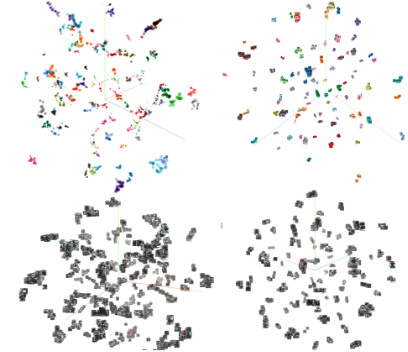
\includegraphics[width=.75\linewidth,keepaspectratio]{data/kaitibaogao/vis2.png}
	\caption{\kaiti 测试集(左图)与训练集合的子集(右图)特征降维可视化。}
	\label{figure:vis2}
\end{figure}

我们也会尝试将在线难样本挖掘用于含有匹配网络的双孪模型。含有匹配网络的双孪模型增大对齐能力的同时也增大了计算量。在这种模型上实现在线难样本挖掘只需要多进行128*128次前向计算(增加1.6s/iter左右的时间),选择最富有信息的样本对即可。这类模型的优点在于可学习的匹配函数,摆脱了欧氏距离的缺点。我们知道目前含有匹配网络的双孪模型较好的水平为80\%(在CUHK03上,cmc-1指标),我们有信心使用在线难样本挖掘将他提升到85.43\%。而用了在线难样本挖掘的三元损失模型(TriHard)只有85\%。因此如果进一步在损失函数、模型结构上扩展,我们也许有机会达到更高的水平。如果按着这一研究方向进行,我们尝试引入一些非线性模型的想法。

在局部特征与全局特征的融合方面,我们会尝试使用Part-reid方法。使用时注意观察TriHard中提到的注意事项会有怎样的影响。比如激活函数的使用,ReLU,L2 Normalize,Sigmoid函数究竟该不该用、用在哪里。小心一些不合理的设置,比如BatchNorm之前和之后同时使用ReLU函数,当模型变得复杂时,很容易出现这些简单的错误。这时候不能归咎于方法不起作用,而应该通过单元测试、输出中间变量可视化等方式找到错误。同时这也有助于我们了解模型的特点和优缺点。

\begin{figure}
	\centering
	\captionsetup{width=.88\linewidth}
	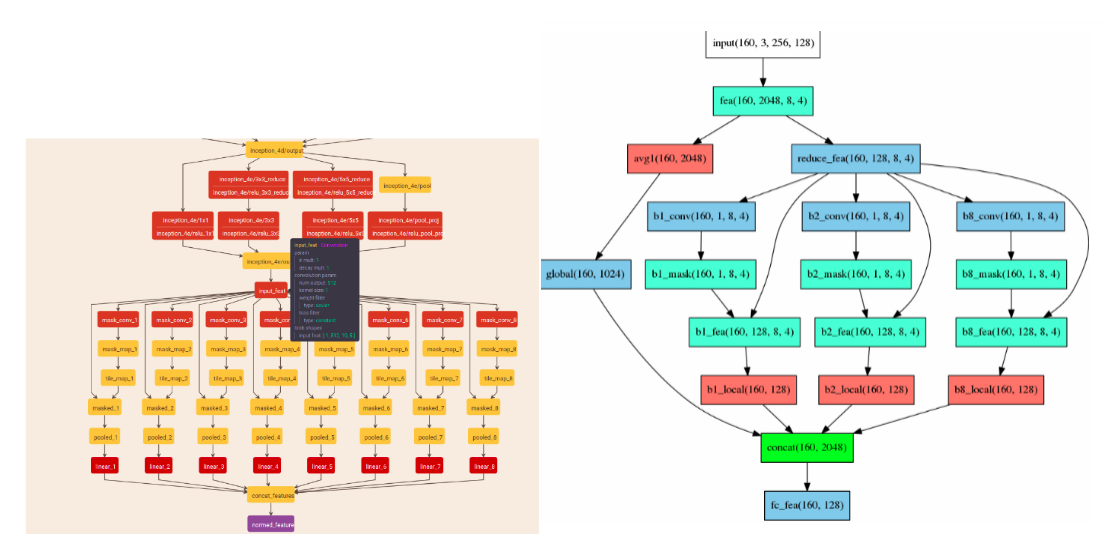
\includegraphics[width=\linewidth,keepaspectratio]{data/kaitibaogao/vis3.png}
	\caption{\kaiti Part-reid的网络结构,左图:论文中的使用的结构。右图:我们计划实现的版本}
	\label{figure:vis3}
\end{figure}

\subsubsection{提出我们的方法}

我们将在观察到的现象的基础上,提出我们的方法。虽然想法很重要,决定了一篇文章是否有影响力,但是目前很难下定论,什么样的想法能够起作用。
按照最初课题的方向,我们可以从GAN、Video的角度着手,比如使用IRGAN选择富有信息的样本,GAN的训练比较困难会遇到训练崩溃的情况,对此一定要耐心调试、多吸取前人的经验。针对Video数据,一方面可以提取时序特征,作为行人的描述子;另一方面,可以将问题转化为multi-shot的问题,考虑每帧图片的质量的基础上进行特征融合。
同时也可以在其他方面着手,比如目前的reid研究都强行将set2set的问题[1]转化为point2point,无论训练还是测试都只比较两张图片的相似度。这才让rerank有机可乘。可以尝试结合NTM将rerank利用上下文信息的步骤端到端地结合到网络中,从而在一定意义上实现自动的single-shot到multi-shot的转换。同时我们也会在选择样本、特征提取、基础卷积模块的设计上着手,选择最有效果的方向深入研究。

\subsection{预期目标}

\begin{enumerate}
	\item 熟悉典型的行人再识别数据集,编写统一整洁的代码,为开源社区做出一份贡献。
	% \item 广泛阅读文献,熟悉典型的行人再识别方法:全面了解行人再识别问题和解决方法。
	\item 通过实验熟悉行人再识别方法,复现最新工作,达到前沿方法的效果。
    \item 在广泛阅读文献的基础上,熟悉典型的行人再识别方法,提出我们创新点。
    \item 完成科研论文撰写,熟悉科研流程,尝试发表。
\end{enumerate}

{
% \renewcommand{\section}[2]{\section*{#2}\addcontentsline{toc}{section}{#2}}
\section{参考文献}
}

\begin{itemize}
	\item [{[}1{]}] Y. Liu, J.Yan, andW. Ouyang. Quality aware network for set to set recognition. arXiv preprint arXiv:1704.03373, 2017
	\item [{[}2{]}] X. Liu, H. Zhao, M. Tian, L. Sheng, J. Shao, S. Yi, J. Yan, and X. Wang. Hydraplus-net: Attentive deep features for pedestrian analysis. 2017.
	\item [{[}3{]}] Zhong, Z., Zheng, L., Cao, D., \& Li, S. (2017). Re-ranking Person Re-identification with k-reciprocal Encoding. \url{http://arxiv.org/abs/1701.08398}
	\item [{[}4{]}] Zheng, L., Yang, Y., \& Hauptmann, A. G. (2016). Person Re-identification: Past, Present and Future. \url{http://arxiv.org/abs/1610.02984}
	\item [{[}5{]}] Wang, J., Wang, B., Zhang, P., \& Zhang, D. (2017). IRGAN : A Minimax Game for Unifying Generative and Discriminative Information Retrieval Models.
\end{itemize}


% 按文章长度需要启用
\ifthenelse{\equal{\zjuside}{T}}{\newpage\mbox{}\thispagestyle{empty}}{}
